\documentclass[12pt, a4paper]{article}

% =========================================================================
% PACKAGES & DOCUMENT GEOMETRY (100% OVERLEAF TEXLIVE COMPATIBLE)
% =========================================================================
\usepackage[utf8]{inputenc}
\usepackage[T1]{fontenc}
\usepackage{helvet}
\renewcommand{\familydefault}{\sfdefault}

\usepackage[margin=1.8cm, headheight=15pt]{geometry}
\usepackage{amsmath}
\usepackage{amssymb}
\usepackage{graphicx}
\usepackage{array}
\usepackage{tabularx}
\usepackage{booktabs}
\usepackage[table]{xcolor}
\usepackage{enumitem}
\usepackage{titlesec}
\usepackage{fancyhdr}
\usepackage{tocloft}
\usepackage{float}
\usepackage{tcolorbox}
\tcbuselibrary{breakable}
\usepackage{hyperref}

% Automatically search both root folder and any images/ subfolder
\graphicspath{{./}{./images/}}

% =========================================================================
% FORMAL ACADEMIC COLOUR PALETTE (DELIVERABLE 1 STYLE)
% =========================================================================
\definecolor{AcademicNavy}{RGB}{20, 42, 74}
\definecolor{AcademicSlate}{RGB}{51, 65, 85}
\definecolor{BorderGray}{RGB}{203, 213, 225}
\definecolor{BgLight}{RGB}{248, 250, 252}
\definecolor{RowAlt}{RGB}{241, 245, 249}

\hypersetup{
    colorlinks=true,
    linkcolor=AcademicNavy,
    urlcolor=AcademicNavy,
    citecolor=AcademicNavy,
    linktoc=all
}

% =========================================================================
% SECTION & HEADER FORMATTING
% =========================================================================
\titleformat{\section}{\Large\bfseries\color{AcademicNavy}}{\thesection.}{0.5em}{}[\vspace{2pt}{\color{AcademicNavy}\titlerule[0.8pt]}]
\titleformat{\subsection}{\large\bfseries\color{AcademicSlate}}{\thesubsection}{0.5em}{}
\titlespacing*{\section}{0pt}{1.4em}{0.7em}
\titlespacing*{\subsection}{0pt}{1.0em}{0.4em}

\renewcommand{\cftsecleader}{\cftdotfill{\cftdotsep}}
\renewcommand{\cftsecfont}{\bfseries\color{AcademicNavy}}
\renewcommand{\cftsecpagefont}{\bfseries\color{AcademicNavy}}

\pagestyle{fancy}
\fancyhf{}
\fancyhead[L]{\small\textcolor{AcademicSlate}{COMP2300 Deliverable 2: Conceptual Design Report}}
\fancyhead[R]{\small\textcolor{AcademicSlate}{Arnav Mishra, Hiranya Makkar, Keshav Singhal}}
\fancyfoot[C]{\small\textcolor{AcademicSlate}{\thepage}}
\renewcommand{\headrulewidth}{0.4pt}

\setlength{\parindent}{0pt}
\setlength{\parskip}{0.55em}
\setlist[itemize]{leftmargin=1.5em, itemsep=0.25em, topsep=0.2em}

% =========================================================================
% SAFE IMAGE RENDERER (AUTOMATICALLY RENDERS pic1.png - pic9.png)
% =========================================================================
\newcommand{\renderpic}[3]{%
    \IfFileExists{#1}{%
        \includegraphics[width=#2, height=#3, keepaspectratio]{#1}%
    }{%
        \fbox{\parbox[c][0.22\textheight][c]{#2}{\centering\small\textbf{Image Ready: \texttt{#1}}\\[4pt]Upload \texttt{#1} to your Overleaf project root to display automatically.}}%
    }%
}

% =========================================================================
% ACADEMIC SPECIFICATION BOX FOR USER STORIES
% =========================================================================
\newtcolorbox{storybox}[2]{
    breakable,
    colback=BgLight,
    colframe=AcademicNavy,
    colbacktitle=AcademicNavy,
    coltitle=white,
    fonttitle=\bfseries\normalsize,
    title={#1 \hfill {\small\normalfont\textcolor{white}{#2}}},
    boxrule=0.7pt,
    arc=2pt,
    left=8pt,
    right=8pt,
    top=6pt,
    bottom=6pt,
    before skip=8pt,
    after skip=8pt
}

\begin{document}

% =========================================================================
% TITLE PAGE BLOCK
% =========================================================================
\begin{center}
    \vspace*{0.5em}
    {\LARGE\bfseries\color{AcademicNavy} Footprint Lens: Contextual Choice Coach}\\[0.5em]
    {\Large\bfseries COMP2300 Deliverable 2: Conceptual Design Report}\\[0.3em]
    {\normalsize\itshape\color{AcademicSlate} Topic 1: Carbon Footprint Awareness and Reduction Tool (Urban India Context)}\\[1.2em]

    \begin{tabular}{ll}
        \textbf{Module:}  & COMP2300 Software Design and Development Project \\
        \textbf{Date:}    & November 2026 \\
        \textbf{Version:} & 2.0 (Final Synchronised Submission) \\
        \textbf{Authors:} & Arnav Mishra (\texttt{am31g25@soton.ac.uk}) \\
                          & Hiranya Makkar (\texttt{hm8g25@soton.ac.uk}) \\
                          & Keshav Singhal (\texttt{ks3e25@soton.ac.uk})
    \end{tabular}
\end{center}
\vspace{0.8em}

% =========================================================================
% TABLE OF CONTENTS (INDEX)
% =========================================================================
{\color{AcademicNavy}\hrule height 0.8pt}
\vspace{0.3em}
\tableofcontents
\vspace{0.5em}
{\color{AcademicNavy}\hrule height 0.8pt}
\newpage

% =========================================================================
% SECTION 1: PROBLEM SPACE ALIGNMENT
% =========================================================================
\section{Problem Space Alignment and Deliverable 1 Traceability}
This conceptual design directly operationalises the 62-word Job to Be Done (JTBD) established in Deliverable 1, maintaining strict traceability to our thematic analysis of interview transcripts \texttt{CF1}--\texttt{CF10}:

\begin{tcolorbox}[colback=BgLight, colframe=AcademicNavy, boxrule=0.7pt, arc=2pt, left=10pt, right=10pt, top=6pt, bottom=6pt]
\textit{``When I want to understand how my everyday routines and household habits affect the environment, I want to see which activities matter most in terms I can picture and which realistic alternatives are open to me, so that I can make changes that fit my budget, safety, rota, and shared home without being misled, lectured, or blamed for constraints I cannot control.''}
\end{tcolorbox}

To ensure full continuity between problem definition and conceptual architecture, our design maps to all six Deliverable 1 personas across three primary stakeholder groups and four operational scenarios:
\begin{itemize}
    \item \textbf{Urban Students and Shared-Housing Youth:} \textbf{P1 Ananya Deshmukh} (Age 21, Pune engineering hostel student navigating 10:30 PM gate curfews, 3 AM exam deliveries, shared floor geysers, and limited mobile data) and \textbf{P2 Karthik Sundaram} (Age 24, Chennai Environmental Science postgraduate requiring transparent Indian coal-grid factors, electronics repair logging, and CSV export alongside a simple view for co-living flatmates).
    \item \textbf{Time-Poor Urban Working Professionals:} \textbf{P3 Rohan Kulkarni} (Age 29, Bengaluru hybrid software engineer seeking 1BHK AC bill benchmarking, smart-plug cut-offs, and non-preachy monthly challenges) and \textbf{P4 Priya Reddy} (Age 31, Hyderabad rotating night-shift nurse requiring safety-locked night cab exemptions and muted daytime sleep windows).
    \item \textbf{Multi-Generational Household Managers and Elders:} \textbf{P5 Sunita Sharma} (Age 46, Noida 3BHK homemaker managing LPG pressure cooking, terrace composting, \textit{kabadiwala} recycling, and teen shower conflicts) and \textbf{P6 Rajeshwar Prasad Verma} (Age 58, Lucknow retired railway official requiring Plain Hindi interfaces, bucket-water metrics, and hourly fan costs).
    \item \textbf{Core Structural Scenarios:} \textbf{SC1} (Noida 3BHK multi-generational utility and water-bucket conflict), \textbf{SC2} (Pune hostel exam-week quick-commerce and shared geyser disaggregation), \textbf{SC3} (Hyderabad night-shift rota scheduling and safety-cab protection), and \textbf{SC4} (Chennai/Bengaluru WFH AC auditing and commute trade-off simulation).
\end{itemize}

% =========================================================================
% SECTION 2: DESIGN CONCEPT GENERATION
% =========================================================================
\section{Design Concept Generation}
In accordance with the COMP2300 Deliverable 2 specification, our team explored three fundamentally distinct interaction paradigms to fulfil our JTBD rather than minor visual variations of a single layout. Each concept was evaluated against our semantic themes (\textbf{S1} Units \& Localisation, \textbf{S2} Overlooked Scope 3 Drivers, \textbf{S3} Ultra-Low-Friction Multilingual UX), latent themes (\textbf{L1} Split-Incentive Tragedy of the Commons, \textbf{L2} Invisible Domestic Policing Labour, \textbf{L3} Safety \& Shift-Work Constraints), and research questions (\textbf{RQ1}--\textbf{RQ3}).

\subsection{Concept A: Passive Ledger (Automated Receipt and Smart-Plug Auditor)}
Concept A operates as a background desktop financial and utility ledger. Rather than prompting users for daily habit check-ins, the system ingests monthly state electricity board PDFs, exported Swiggy, Zomato, and Amazon order history CSVs, and automated smart-plug wattage logs to compile an retrospective end-of-month carbon and Rupee audit.
\begin{itemize}
    \item \textbf{Operational Mechanics:} Users drag-and-drop monthly billing statements into a parser table. The system applies top-down Input-Output Analysis (IOA) spend multipliers to categorise food delivery packaging, apparel purchases, and appliance kWh usage, producing a monthly financial-environmental balance sheet tailored to \textbf{P3 Rohan} (\texttt{CF2}) and \textbf{P2 Karthik} (\texttt{CF4}).
    \item \textbf{Critical Limitations and Rejection Rationale:} While Concept A reduces daily typing for tech-savvy professionals, it fails our core accessibility and scope criteria. First, it alienates \textbf{P1 Ananya} (\texttt{CF1}) and \textbf{P6 Rajeshwar} (\texttt{CF8}), who do not export e-commerce CSV files or own smart-home telemetry hardware. Second, automated bank and order scraping violates Epic \textbf{E14} (\textit{Won't Have: external account scraping and cloud dependencies in v1.0}). Third, retrospective end-of-month audits provide zero point-of-decision guidance when a user is deciding between a solo cab and a Metro ride (\textbf{SC4}).
\end{itemize}

\subsection{Concept B: Social Kiosk (Communal Household and Hostel Challenge Board)}
Concept B reframes carbon tracking as a shared, ambient household kiosk designed for a family tablet or co-living common-room monitor. It focuses exclusively on collective resource consumption, converting shared electricity bills and municipal water-tanker deliveries into room-by-room splits and competitive household leaderboards.
\begin{itemize}
    \item \textbf{Operational Mechanics:} Household members log shower durations, geyser timer activations, and AC hours onto a central floor board. The interface visualises communal totals in 15-litre water buckets and Rupees, ranking flatmates or family members on a weekly efficiency leaderboard to address \textbf{P5 Sunita}'s (\texttt{CF3}) frustration with unmonitored teen showers in \textbf{SC1}.
    \item \textbf{Critical Limitations and Rejection Rationale:} Despite addressing shared water and energy visibility (\textbf{L2}), Concept B introduces severe socio-technical risks. Publicly ranking individuals on a communal board violates Epic \textbf{E13} (\textit{Won't Have: forced roommate bill-splitting and public shaming leaderboards}) and fails \textbf{RQ3}. In shared student hostels (\textbf{SC2}) or co-living flats (\texttt{CF10}), exposing individual usage without voluntary consent triggers interpersonal conflict. Furthermore, Concept B provides no support for solo rotating shift workers like \textbf{P4 Priya} (\textbf{SC3}) and lacks the granular formula provenance required by \textbf{P2 Karthik} (\textbf{E2}).
\end{itemize}

\subsection{Concept C: Hybrid Simulator (Dual-Mode Adaptive Companion --- Selected)}
Concept C synthesises low-friction daily logging with an interactive decision sandbox inside a 100\% offline-first desktop application. It pairs a \textbf{Simple Companion View} (driven by 2-tap presets and Plain Hindi/vernacular toggles) with an on-demand \textbf{Detailed Researcher Audit View} (providing editable emission factors and local CSV export).
\begin{itemize}
    \item \textbf{Operational Mechanics:} Users define their session scope and safety/shift constraints at entry (\textbf{State P0}), log routines in under 60 seconds using 2-tap preset cards or single-field quantities (\textbf{State P1}), and immediately inspect their impact paired with Rupees, 15L water buckets, and city bus trips alongside a live ``What-If'' habit swap slider (\textbf{State P2}). Domain experts can open the Provenance Inspector (\textbf{State P3}) to edit the Central Electricity Authority (CEA) grid factor ($0.716\text{ kg CO}_2\text{/kWh}$) or local tariff ($\text{Rs. }8.00\text{/kWh}$). Crucially, Concept C enforces a \textbf{Constraint Shield} (\textbf{State P4}) that exempts night-shift safety cabs and daytime sleep AC from moralising penalties (\textbf{L3}), records traditional repair and composting habits descriptively without fabricating fake carbon offsets (\textbf{State P5}), and defaults shared household bills to communal totals with strictly voluntary opt-in attribution (\textbf{State P6}).
    \item \textbf{Selection Justification:} Concept C is the only paradigm that resolves all four scenarios (\textbf{SC1}--\textbf{SC4}) and serves all six personas (\textbf{P1}--\textbf{P6}) via progressive disclosure. It directly answers \textbf{RQ1} (tangible unit comprehension), \textbf{RQ2} (2-tap low-friction logging), and \textbf{RQ3} (non-policing household boundaries) while remaining 100\% implementable in standalone Java and JavaFX with local JSON persistence.
\end{itemize}

% =========================================================================
% SECTION 3: CONCEPT SELECTION ANALYSIS (MCDM)
% =========================================================================
\section{Concept Selection Analysis (MCDM)}
Table \ref{tab:mcdm} presents the Multi-Criteria Decision Analysis (MCDM) used to evaluate the three concepts against weighted engineering and human-factors criteria derived from Deliverable 1.

\begin{table}[H]
\centering
\small
\renewcommand{\arraystretch}{1.45}
\begin{tabularx}{\textwidth}{@{} >{\bfseries}p{3.0cm} c X X X @{}}
\toprule
\rowcolor{AcademicNavy}
\textcolor{white}{Criterion} & \textcolor{white}{Weight} & \textcolor{white}{Concept A: Passive Ledger} & \textcolor{white}{Concept B: Social Kiosk} & \textcolor{white}{Concept C: Hybrid Simulator} \\
\midrule
D1 Must Epics (E1--E5) & 25\% & \textbf{2.0 / 5.0}\newline Fails E3 safety shields and E5 2-tap manual entry. & \textbf{3.0 / 5.0}\newline Supports buckets (E1) but weak on E2 formula audit and E3. & \textbf{5.0 / 5.0}\newline Fully satisfies E1--E5 offline with 2-tap presets and shields. \\
\rowcolor{RowAlt}
Persona \& Scenario Fit & 25\% & \textbf{2.5 / 5.0}\newline Excludes P1 (student) and P6 (elder) who lack CSVs. & \textbf{3.5 / 5.0}\newline Fits SC1 families but fails solo shift nurse P4 (SC3). & \textbf{4.5 / 5.0}\newline Serves P1--P6 across SC1--SC4 via dual-mode views. \\
JavaFX Offline Feasibility & 20\% & \textbf{2.5 / 5.0}\newline Bill/PDF parsing is brittle and risks E14 scope creep. & \textbf{2.5 / 5.0}\newline Multi-device sync adds unnecessary network overhead. & \textbf{5.0 / 5.0}\newline Clean JavaFX MVVM + Strategy pattern + local JSON. \\
\rowcolor{RowAlt}
Transparency \& Provenance & 15\% & \textbf{3.0 / 5.0}\newline Spend multipliers act as an opaque black box. & \textbf{3.0 / 5.0}\newline Prioritises gamified badges over visible assumptions. & \textbf{5.0 / 5.0}\newline Dedicated State P3 table with editable grid/tariff inputs. \\
Socio-Technical Risk Profile & 15\% & \textbf{3.0 / 5.0}\newline High privacy concern around financial statement import. & \textbf{2.0 / 5.0}\newline High risk of roommate policing friction (violates E13). & \textbf{4.5 / 5.0}\newline Voluntary opt-in (P6) and no fake offsets (P5) minimise risk. \\
\midrule
\textbf{Weighted Total} & \textbf{100\%} & \textbf{2.55 / 5.00} & \textbf{2.90 / 5.00} & \textbf{4.78 / 5.00 (Selected)} \\
\bottomrule
\end{tabularx}
\caption{Multi-Criteria Decision Matrix justifying the selection of Concept C.}
\label{tab:mcdm}
\end{table}

\newpage

% =========================================================================
% SECTION 4: DETAILED USER STORY REGISTER (FULL-SPACE CARDS)
% =========================================================================
\section{Detailed User Story Register (Epics E1--E14)}
Concept C is decomposed into twelve granular user story specifications covering all fourteen Deliverable 1 Epics (\textbf{E1}--\textbf{E14}). Each specification defines the MoSCoW priority, target personas, scenario links, and testable Behavior-Driven Development (BDD) acceptance criteria (\textit{Given / When / Then}) to govern Deliverable 3 evaluation and Deliverables 4--6 JUnit verification.

\begin{storybox}{US01 (Epic E1): Tangible Dual-Unit Metric Translation}{MoSCoW: Must Have | Personas: P1, P3, P5, P6 | Scenarios: SC1--SC4}
\textbf{User Story:} As an urban Indian user unfamiliar with abstract climate metrics, I want every emission estimate paired with familiar physical and financial equivalents (Indian Rupees, 15-litre water buckets, fan/AC hours, and city bus trips) alongside $\text{kg CO}_2\text{e}$, so that I can immediately picture the real-world scale of my household and commuting routines.
\begin{itemize}
    \item \textbf{Given} a valid routine quantity is entered or selected via preset in State P1 (e.g., $168.0\text{ kWh}$ monthly electricity),
    \item \textbf{When} the calculation engine executes the emission conversion strategy,
    \item \textbf{Then} State P2 displays the primary $\text{kg CO}_2\text{e}$ result ($120.29\text{ kg CO}_2\text{e}$) paired side-by-side with exact local equivalents ($\text{Rs. }1,344$ tariff cost and $534$ city bus trips) without requiring a secondary menu click.
\end{itemize}
\end{storybox}

\begin{storybox}{US02 (Epic E2): Transparent Assumption Inspection and Live Editing}{MoSCoW: Must Have | Personas: P2, P3, P5 | Scenarios: SC2, SC4}
\textbf{User Story:} As an evidence-conscious researcher or analytical householder, I want to inspect and edit the underlying conversion assumptions (regional CEA coal-grid factor, electricity tariff rate, and mathematical formula), so that I can verify where estimates come from and calibrate them to my state electricity board bill.
\begin{itemize}
    \item \textbf{Given} a calculated routine footprint in State P2,
    \item \textbf{When} the user navigates to State P3 (Assumptions Inspector) and modifies an editable parameter (e.g., changing the grid factor from $0.716$ to $0.820\text{ kg CO}_2\text{/kWh}$ or tariff from $\text{Rs. }8.00\text{/kWh}$) and clicks \textit{Apply \& Recalculate},
    \item \textbf{Then} the displayed formula ($\text{Qty} \times \text{Factor} = \text{kg CO}_2\text{e}$) and all dependent dashboard metrics update instantaneously across the session.
\end{itemize}
\end{storybox}

\begin{storybox}{US03 (Epic E3): Structural Constraint Shield for Safety and Shift Routines}{MoSCoW: Must Have | Personas: P1, P4 | Scenarios: SC2, SC3}
\textbf{User Story:} As a night-shift healthcare worker or student subject to hostel curfews, I want to flag non-negotiable routines (such as late-night safety cabs or post-shift daytime sleep AC) as protected necessities, so that the tool never penalises or lectures me for structural constraints outside my control.
\begin{itemize}
    \item \textbf{Given} the user checks the \textit{Protected Health/Safety Routine} checkbox in State P0,
    \item \textbf{When} the user views the Constraint Shield action screen in State P4,
    \item \textbf{Then} the interface displays a prominent notice confirming that substitution prompts are disabled for the protected routine, applies zero guilt penalties, and offers Choose / Defer / Not Feasible controls for optional non-protected swaps.
\end{itemize}
\end{storybox}

\begin{storybox}{US04 (Epic E4): Descriptive Circularity and Low-Waste Habit Recognition}{MoSCoW: Must Have | Personas: P1--P6 | Scenarios: SC1, SC2}
\textbf{User Story:} As a householder practising traditional Indian frugality (electronics repair, terrace composting, bucket baths, and \textit{kabadiwala} scrap recycling), I want circular habits recorded descriptively on my summary without inventing fake carbon offset numbers, so that my sustainable practices are recognised honestly.
\begin{itemize}
    \item \textbf{Given} the user selects a circularity category (e.g., \textit{Phone Repair / Composting}) in State P5,
    \item \textbf{When} the habit is saved with \textit{Credited on Household Summary} checked,
    \item \textbf{Then} the system logs the practice as a verified descriptive badge explicitly labelled \textit{Status: Estimate Unavailable (No Fake Offsets)} and never subtracts fabricated $\text{kg CO}_2\text{e}$ deductions from direct energy totals.
\end{itemize}
\end{storybox}

\begin{storybox}{US05 (Epic E5): Offline 2-Tap Preset Logger and Plain Hindi Toggle}{MoSCoW: Must Have | Personas: P1, P4, P6 | Scenarios: SC1, SC2, SC3}
\textbf{User Story:} As a time-poor student or non-English-speaking elder with a limited mobile data plan, I want 2-tap routine preset cards and an instant English / Plain Hindi language selector that works 100\% offline, so that I can complete a check-in in under 60 seconds without data charges or 40-question forms.
\begin{itemize}
    \item \textbf{Given} the application is running with zero network connectivity,
    \item \textbf{When} the user selects \textit{Plain Hindi} or \textit{English} in State P0 and taps a single preset card in State P1 (\textit{Delivery Box}, \textit{1.5 kW AC}, or \textit{2 kW Geyser}),
    \item \textbf{Then} the quantity and unit auto-fill immediately and transition to the contextual result in $\le 2$ taps and under 60 seconds.
\end{itemize}
\end{storybox}

\begin{storybox}{US06 (Epic E6): Side-by-Side What-If Habit Swap Simulator}{MoSCoW: Should Have | Personas: P1, P3, P5 | Scenarios: SC1, SC3, SC4}
\textbf{User Story:} As a decision-maker comparing everyday alternatives, I want an interactive What-If slider that previews the exact monthly Rupee and $\text{kg CO}_2\text{e}$ savings of a realistic adjustment (such as cutting WFH AC runtime by 1 hour or swapping one car commute to the Metro), so that I can evaluate trade-offs before committing.
\begin{itemize}
    \item \textbf{Given} a baseline routine calculation in State P2 ($168.0\text{ kWh} = 120.29\text{ kg CO}_2\text{e}$),
    \item \textbf{When} the user adjusts the \textit{What-If Swap Simulator} slider (\textit{Cut 1.5 kW WFH AC 1 hr early}),
    \item \textbf{Then} the simulator dynamically displays the net monthly reduction (\textit{Saves $15.04\text{ kg CO}_2\text{e}$ \& $\text{Rs. }168\text{/mo}$}) alongside the baseline figure.
\end{itemize}
\end{storybox}

\begin{storybox}{US07 (Epic E7): Shared Household Boundary with Voluntary Opt-In}{MoSCoW: Should Have | Personas: P1, P2, P3, P5, P6 | Scenarios: SC1, SC2}
\textbf{User Story:} As a resident in a multi-generational home or shared student flat, I want shared utility bills displayed as a communal total by default with a strictly voluntary opt-in toggle for my own room share, so that we can coordinate household reductions without policing or blaming flatmates.
\begin{itemize}
    \item \textbf{Given} \textit{Household Scope} is selected for a shared bill ($168\text{ kWh}$) in State P6,
    \item \textbf{When} the Shared Household Boundary view loads,
    \item \textbf{Then} it displays the \textit{Communal Total (Default)} alongside the rule \textit{``Shared bills do not equal personal footprints''}, permits the active user to check \textit{Opt in to show my room AC share}, blocks forced attribution for flatmates, and provides a shareable Hindi/Marathi floor card.
\end{itemize}
\end{storybox}

\begin{storybox}{US08 (Epic E8): Non-Judgmental Monthly Summary and Single Challenge}{MoSCoW: Should Have | Personas: P1, P3, P5 | Scenarios: SC3, SC4}
\textbf{User Story:} As a user fatigued by moralising eco-guilt, I want a clean monthly category breakdown paired with a single optional monthly challenge (such as keeping a smartphone an extra year or batching grocery orders), so that I can track progress without punitive streak counters.
\begin{itemize}
    \item \textbf{Given} multiple routines are logged across a monthly cycle,
    \item \textbf{When} the monthly summary is viewed,
    \item \textbf{Then} emissions and Rupee costs are grouped by domain (Energy, Mobility, Delivery/Packaging, Circularity) with zero red shaming badges or streak penalties.
\end{itemize}
\end{storybox}

\begin{storybox}{US09 (Epic E9): Researcher Audit View and Local CSV Export}{MoSCoW: Should Have | Personas: P2 | Scenarios: SC2, SC4}
\textbf{User Story:} As an environmental science postgraduate, I want to export session logs and active assumption parameters to a local CSV file, so that I can perform regional sensitivity analyses in external research tools without cloud dependencies.
\begin{itemize}
    \item \textbf{Given} active session calculations and provenance parameters in State P3,
    \item \textbf{When} the user clicks \textit{Export CSV Data},
    \item \textbf{Then} the system writes a structured \texttt{.csv} file containing quantities, units, grid factors, tariffs, and calculated $\text{kg CO}_2\text{e}$ directly to the local filesystem.
\end{itemize}
\end{storybox}

\begin{storybox}{US10 (Epics E10, E11, E12): Rota Quiet Windows, Local Flat Benchmarks, and Smart-Plug Timers}{MoSCoW: Could Have | Personas: P3, P4 | Scenarios: SC3, SC4}
\textbf{User Story:} As a shift worker or hybrid engineer, I want optional rota-aware notification muting during daytime sleep hours (\textbf{E10}), static reference-flat benchmarks for Indian 1BHK/2BHK/3BHK homes (\textbf{E11}), and simulated smart-plug cut-off scheduling (\textbf{E12}), so that advanced automation can be layered onto the core tracker in later increments.
\begin{itemize}
    \item \textbf{Given} a user enables night-shift rota muting in State P0 or selects an AC cut-off swap in State P4,
    \item \textbf{When} daytime sleep hours occur or the benchmark view is inspected,
    \item \textbf{Then} daytime alerts remain suppressed and WFH appliance loads are compared against static local flat baselines.
\end{itemize}
\end{storybox}

\begin{storybox}{US11 \& US12 (Epics E13 \& E14): Explicitly Excluded v1.0 Scope}{MoSCoW: Won't Have (v1.0) | Personas: All (P1--P6) | Scenarios: SC1--SC4}
\textbf{Excluded Capabilities:}
\begin{itemize}
    \item \textbf{Epic E13 (Social Shaming \& Forced Splits):} Public competitive leaderboards, mandatory per-person bill splitting without consent, and red penalty scores are strictly excluded to protect household harmony (\textbf{L1, L2, RQ3}).
    \item \textbf{Epic E14 (Speculative Cloud AI, Bank Scraping \& Unverified Offsets):} Live bank/credit-card statement scraping, cloud vision food-photo APIs, building construction material LCA, and commercial carbon-offset marketplaces are excluded from v1.0 to guarantee 100\% offline privacy and mathematical honesty.
\end{itemize}
\end{storybox}

\clearpage

% =========================================================================
% SECTION 5: LOW-FIDELITY PROTOTYPE & WALKTHROUGH
% =========================================================================
\section{Low-Fidelity Conceptual Prototype and State Walkthrough}
In strict compliance with the COMP2300 Deliverable 2 rubric, our prototype is constructed strictly as an unpolished, monochromatic low-fidelity wireframe flow (\textbf{States P0--P6}). No backend programming, high-fidelity CSS theming, or executable business logic was prematurely built at this stage. Instead, the wireframes isolate the core interaction architecture required to evaluate our three research questions prior to Deliverable 4 JavaFX development:

\begin{enumerate}[leftmargin=1.8em, itemsep=0.3em]
    \item \textbf{Master Architectural Flow (\texttt{pic1.png}):} Maps the complete 7-state state-machine topology on a single blueprint canvas, demonstrating how users progress from initial scope and language selection (\textbf{P0}) to 2-tap preset entry (\textbf{P1}), contextual feedback (\textbf{P2}), and specialised branching into provenance auditing (\textbf{P3}), safety-shield actions (\textbf{P4}), circular habit logging (\textbf{P5}), and shared household boundaries (\textbf{P6}).
    \item \textbf{State P0 --- Entry \& Scope (\texttt{pic2.png}):} Resolves \textbf{Epic E5} and \textbf{Epic E3} at session start. Users select their interface language (\textit{English / Plain Hindi}) via a top-level dropdown and configure boundary checkboxes for \textit{Household Scope} and \textit{Protected Health/Safety Routine} before advancing.
    \item \textbf{State P1 --- Quantity Logger (\texttt{pic3.png}):} Operationalises \textbf{RQ2} (low-friction entry) and \textbf{Epic E5}. Users can bypass manual typing entirely by clicking one of three prominent \textit{2-Tap Presets} (\textit{Delivery Box}, \textit{1.5 kW AC}, \textit{2 kW Geyser}) to auto-populate standard quantities, or enter a single numeric value ($168.0\text{ kWh}$) in the manual input box.
    \item \textbf{State P2 --- Result \& What-If Simulator (\texttt{pic4.png}):} Operationalises \textbf{RQ1} (unit comprehension), \textbf{Epic E1}, and \textbf{Epic E6}. The primary estimate ($120.29\text{ kg CO}_2\text{e}$) is immediately contextualised beside $\text{Rs. }1,344\text{ saved | }534\text{ city bus trips}$. Directly beneath, the interactive \textit{What-If Swap Simulator} slider previews the impact of cutting WFH AC usage 1 hour early (\textit{Saves $15.04\text{ kg CO}_2\text{e}$ \& $\text{Rs. }168\text{/mo}$}), with bottom navigation icons linking to \textit{Assumptions Audit}, \textit{Action Shield}, and \textit{Shared Hub}.
    \item \textbf{State P3 --- Assumptions Inspector (\texttt{pic5.png}):} Operationalises \textbf{Epic E2} and \textbf{Epic E9} for \textbf{P2 Karthik}. Displays a structured \textit{Provenance Table} exposing the editable \textit{Grid Factor} ($0.716\text{ kg CO}_2\text{/kWh}$), editable \textit{Tariff Rate} ($\text{Rs. }8.00\text{/kWh}$), and explicit \textit{Formula} ($\text{Qty} \times \text{Factor} = \text{kg CO}_2\text{e}$), paired with \textit{Apply \& Recalculate} and \textit{Export CSV Data} controls.
    \item \textbf{State P4 --- Constraint Shield (\texttt{pic6.png}):} Operationalises \textbf{Epic E3} and Latent Theme \textbf{L3} for \textbf{P4 Priya} and \textbf{P1 Ananya}. When a routine is flagged as a health or safety necessity, a prominent banner states: \textit{``Safety Necessity Flagged. Action disabled. Zero penalty applied.''} For non-locked routines, users retain full agency via three non-judgmental action buttons: \textit{Choose}, \textit{Defer}, or \textit{Not Feasible}.
    \item \textbf{State P5 --- Circular Record (\texttt{pic7.png}):} Operationalises \textbf{Epic E4} and \textbf{Epic E14}. Logs circular practices (\textit{Phone Repair / Composting}) with a transparent \textit{Status Badge} (\textit{Status: Estimate Unavailable --- No Fake Offsets}) and a household summary credit toggle, preventing greenwashing while validating elder and student reuse habits.
    \item \textbf{State P6 --- Shared Household Boundary (\texttt{pic8.png}):} Operationalises \textbf{RQ3} and \textbf{Epic E7}. Displays the \textit{Communal Total (Default)} ($168\text{ kWh}$) alongside the explicit boundary rule (\textit{``Shared bills do not equal personal footprints''}). Individual room attribution is governed by a voluntary opt-in checkbox (\textit{Opt in to show my room AC share}), while forced attribution for flatmates is permanently disabled, accompanied by a \textit{Share Hindi/Marathi Floor Card} button.
\end{enumerate}

\newpage

% =========================================================================
% PROTOTYPE PAGE 1: MASTER ARCHITECTURAL FLOW (1 IMAGE)
% =========================================================================
\begin{figure}[H]
    \centering
    \renderpic{pic1.png}{0.98\textwidth}{0.78\textheight}
    \caption{Master Architectural Wireframe Grid (\texttt{pic1.png}) showing the complete offline state topology across States P0--P6.}
    \label{fig:master-wireframe}
\end{figure}

\newpage

% =========================================================================
% PROTOTYPE PAGE 2: STATES P0, P1, P2, P3 (EXACTLY 4 IMAGES)
% =========================================================================
\begin{figure}[H]
    \centering
    \begin{minipage}[t]{0.48\textwidth}
        \centering
        \renderpic{pic2.png}{\linewidth}{0.37\textheight}
        \vspace{2pt}
        {\footnotesize \textbf{(a) State P0 (\texttt{pic2.png}):} Entry, Language \& Scope.}
    \end{minipage}\hfill
    \begin{minipage}[t]{0.48\textwidth}
        \centering
        \renderpic{pic3.png}{\linewidth}{0.37\textheight}
        \vspace{2pt}
        {\footnotesize \textbf{(b) State P1 (\texttt{pic3.png}):} 2-Tap Presets \& Manual Logger.}
    \end{minipage}

    \vspace{0.6cm}

    \begin{minipage}[t]{0.48\textwidth}
        \centering
        \renderpic{pic4.png}{\linewidth}{0.37\textheight}
        \vspace{2pt}
        {\footnotesize \textbf{(c) State P2 (\texttt{pic4.png}):} Result \& What-If Simulator.}
    \end{minipage}\hfill
    \begin{minipage}[t]{0.48\textwidth}
        \centering
        \renderpic{pic5.png}{\linewidth}{0.37\textheight}
        \vspace{2pt}
        {\footnotesize \textbf{(d) State P3 (\texttt{pic5.png}):} Provenance \& Assumptions Audit.}
    \end{minipage}
    \caption{Low-fidelity wireframes for States P0, P1, P2, and P3 enforcing Epics E1, E2, E5, E6, and E9.}
    \label{fig:wireframes-p0-p3}
\end{figure}

\newpage

% =========================================================================
% PROTOTYPE PAGE 3: STATES P4, P5, P6 (EXACTLY 3 IMAGES)
% =========================================================================
\begin{figure}[H]
    \centering
    \begin{minipage}[t]{0.48\textwidth}
        \centering
        \renderpic{pic6.png}{\linewidth}{0.37\textheight}
        \vspace{2pt}
        {\footnotesize \textbf{(a) State P4 (\texttt{pic6.png}):} Constraint Shield \& Agency Options.}
    \end{minipage}\hfill
    \begin{minipage}[t]{0.48\textwidth}
        \centering
        \renderpic{pic7.png}{\linewidth}{0.37\textheight}
        \vspace{2pt}
        {\footnotesize \textbf{(b) State P5 (\texttt{pic7.png}):} Descriptive Circular Habit Record.}
    \end{minipage}

    \vspace{0.6cm}

    \begin{minipage}[t]{0.52\textwidth}
        \centering
        \renderpic{pic8.png}{\linewidth}{0.37\textheight}
        \vspace{2pt}
        {\footnotesize \textbf{(c) State P6 (\texttt{pic8.png}):} Shared Household Boundary \& Voluntary Opt-In.}
    \end{minipage}
    \caption{Low-fidelity wireframes for States P4, P5, and P6 enforcing Epics E3, E4, E7, E13, and E14.}
    \label{fig:wireframes-p4-p6}
\end{figure}

\clearpage

% =========================================================================
% SECTION 6: EVALUATION PLAN, PROJECT MANAGEMENT & AGILE REFLECTION
% =========================================================================
\section{Formative Evaluation Plan and Agile Project Management}

\subsection{Formative Evaluation Plan (Testing RQ1--RQ3)}
To prepare for Deliverable 3, States P0--P6 are structured to support a lab-based think-aloud usability evaluation with external COMP2300 participants (strictly avoiding heuristic evaluation or sensitive personal data collection):
\begin{itemize}
    \item \textbf{Task 1 --- Low-Friction Preset Logging (\textbf{RQ2}, States P0--P1):} Participants select \textit{Plain Hindi} or \textit{English} in State P0 and log a $168.0\text{ kWh}$ home electricity routine using State P1 presets. \textit{Target Metric:} Task completion in $\le 60\text{ seconds}$ and $\le 2$ state transitions.
    \item \textbf{Task 2 --- Tangible Equivalent \& What-If Comprehension (\textbf{RQ1}, States P2--P3):} Participants inspect the dual-unit output ($\text{Rs. }1,344$ and $534$ bus trips), use the What-If slider to evaluate cutting WFH AC runtime by 1 hour, and verify the $0.716\text{ kg CO}_2\text{/kWh}$ grid factor in State P3. \textit{Target Metric:} $100\%$ accuracy in identifying the highest-saving action and its underlying formula.
    \item \textbf{Task 3 --- Constraint Shield \& Shared Boundary Navigation (\textbf{RQ3}, States P4--P6):} Participants verify that a safety-flagged night cab triggers zero penalty in State P4, log a phone repair in State P5, and configure voluntary room AC opt-in in State P6. \textit{Target Metric:} Zero perceived flatmate policing friction in post-task debriefs.
\end{itemize}

\subsection{Sprint 1 Plan, Risk Register, and Retrospective Reflection}
Table \ref{tab:risk-log} summarises our active project risk register and mitigation controls moving into Deliverable 3 and Sprint 1 (Deliverable 4).

\begin{table}[H]
\centering
\small
\renewcommand{\arraystretch}{1.35}
\begin{tabularx}{\textwidth}{@{} p{1.2cm} p{3.4cm} c X @{}}
\toprule
\rowcolor{AcademicNavy}
\textcolor{white}{\textbf{ID}} & \textcolor{white}{\textbf{Identified Risk}} & \textcolor{white}{\textbf{Severity}} & \textcolor{white}{\textbf{Mitigation \& Contingency Strategy}} \\
\midrule
\textbf{R1} & D1-to-D2 requirement drift across personas or epics. & High & Enforced a 1-to-1 traceability matrix mapping all 6 personas (P1--P6), 4 scenarios (SC1--SC4), and 14 epics (E1--E14) directly to UoS GitLab Issues. \\
\rowcolor{RowAlt}
\textbf{R2} & Prototype fidelity penalty (looking too polished or coded in D2). & High & Used strictly monochromatic, low-fidelity conceptual wireframes (\texttt{pic1}--\texttt{pic8}) with zero application coding in D2. \\
\textbf{R3} & Uneven GitLab commit visibility or member unavailability in Sprint 1. & Medium & Partitioned MVVM architecture into independent layers (Models/JSON, FXML Views, ViewModels/JUnit) on separate GitLab feature branches with mandatory peer Merge Requests. \\
\bottomrule
\end{tabularx}
\caption{Deliverable 2 Risk Register and Mitigation Controls.}
\label{tab:risk-log}
\end{table}

\textbf{Product Reflection (Sprint Review):} Converging on Concept C resolved the core design tension uncovered in Deliverable 1: serving low-literacy or time-poor users (\textbf{P1, P4, P6}) alongside rigorous domain researchers (\textbf{P2}). Separating the 2-tap preset flow (States P0--P2) from the on-demand Provenance Inspector (State P3) achieved progressive disclosure without cluttering the primary interface.

\textbf{Process Reflection (Sprint Retrospective):} During early D2 drafting, our team noticed a risk of compressing our six D1 personas into generic archetypes. Conducting a formal D1-to-D2 synchronisation audit allowed us to restore full coverage of all 14 Epics (\textbf{E1}--\textbf{E14}) and transition our backlog tracking into milestone-tagged UoS GitLab Issues ahead of Deliverable 3.

% =========================================================================
% SECTION 7: SYSTEM ARCHITECTURE AND TECHNICAL DESIGN BRIEF (PIC 9)
% =========================================================================
\section{System Architecture and Technical Design Brief}
To guarantee long-term maintainability and strictly enforce the offline-first privacy constraints defined in Epics \textbf{E5} and \textbf{E14}, the target Java 21 and JavaFX application is architected using a modular \textbf{Model-View-ViewModel (MVVM)} pattern coupled with the \textbf{Strategy Pattern} (Figure \ref{fig:system-architecture}):

\begin{itemize}
    \item \textbf{Presentation Layer (JavaFX \texttt{.fxml} Views):} Consists of passive UI views (\texttt{SimpleDashboardView}, \texttt{HouseholdHubView}, \texttt{AssumptionsAuditView}) that bind declaratively to ViewModel `ObservableProperties`. Toggling between English and Plain Hindi (`ResourceBundle`) or adjusting the What-If slider updates UI labels reactively without manual thread redraws.
    \item \textbf{ViewModel Layer (State \& Boundary Enforcement):} Mediates UI state (\texttt{DashboardViewModel}, \texttt{HouseholdViewModel}, \texttt{AuditViewModel}) and enforces socio-technical rules—such as masking individual room attributions in State P6 unless the voluntary `isAttributionOptedIn()` property is explicitly set to `true`, and suppressing action nudges when the State P0 safety-lock flag is active.
    \item \textbf{Model \& Service Layer (Strategy Pattern --- Open/Closed Principle):} An `EmissionCalculationStrategy` interface abstracts domain logic across concrete implementations (`ApplianceWaterCalculator`, `TransportCalculator`, and `QuickCommerceCalculator`). These calculators read visible parameters ($0.716\text{ kg CO}_2\text{/kWh}$ grid factor, $\text{Rs. }8.00\text{/kWh}$ tariff) from `AssumptionsConfig` and pass results to `UnitEquivalencyConverter` to generate Rupee, bucket, and bus-trip equivalents.
    \item \textbf{Data Persistence Layer (100\% Offline Local Storage):} `LocalRepository` serialises user logs and custom assumption configurations into local JSON files via Jackson/Gson and writes local CSV exports in State P3, ensuring zero external network calls or mobile data consumption.
\end{itemize}

\begin{figure}[H]
    \centering
    \renderpic{pic9.png}{0.92\textwidth}{0.48\textheight}
    \caption{System Architecture Diagram (\texttt{pic9.png}) illustrating the offline-first JavaFX MVVM layers, Strategy Pattern calculation engine, and local JSON/CSV persistence.}
    \label{fig:system-architecture}
\end{figure}

\end{document}\begin{figure}
    \centering
    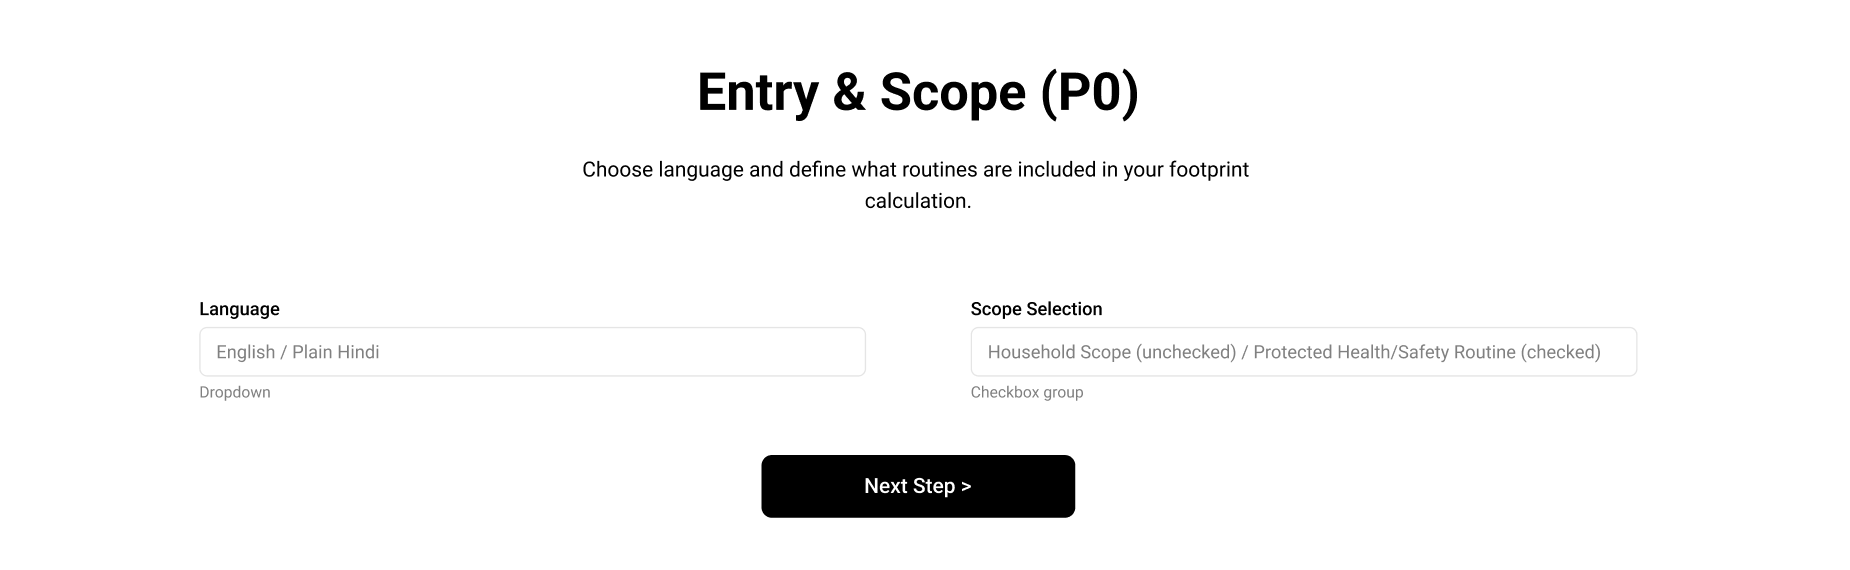
\includegraphics[width=0.5\linewidth]{pic2.png}
    \caption{Enter Caption}
\begin{figure}
        \centering
        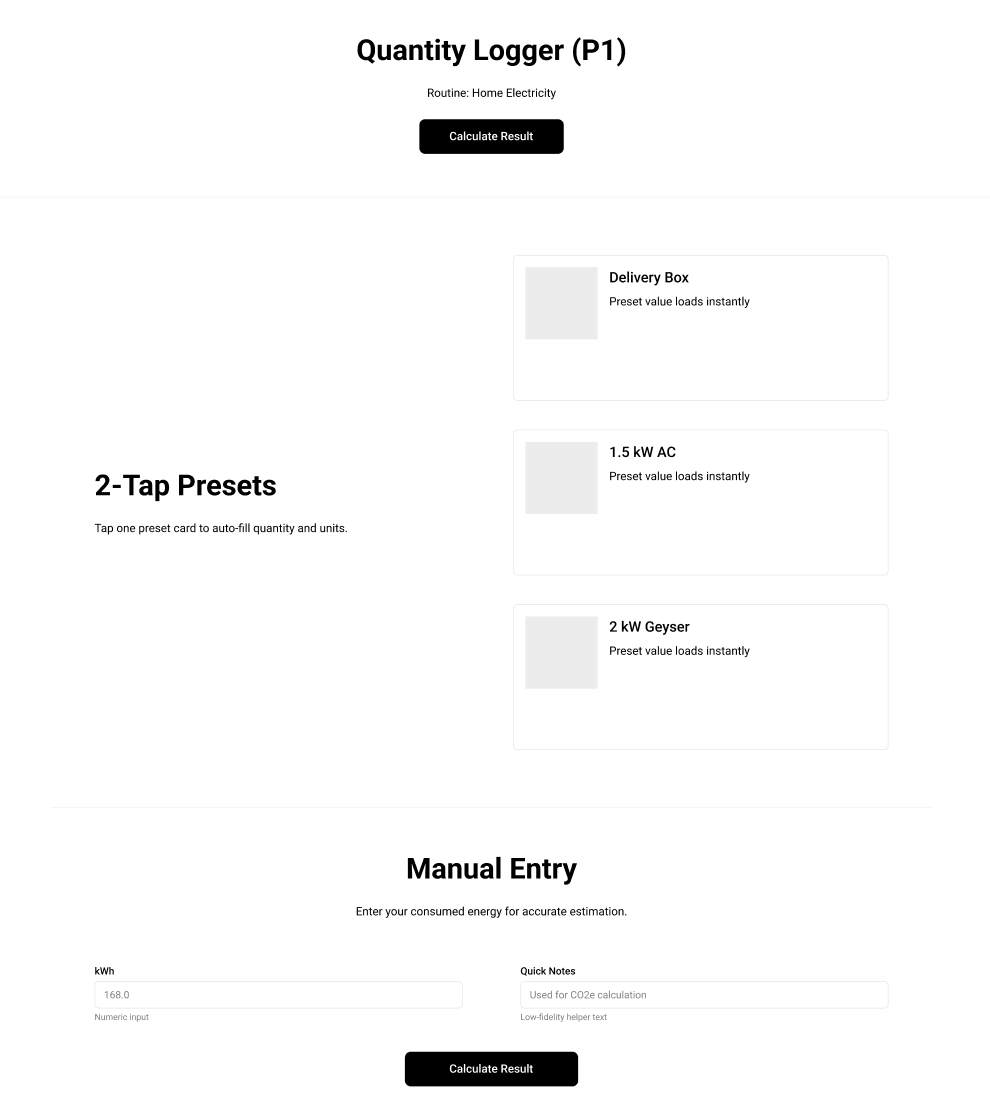
\includegraphics[width=0.5\linewidth]{pic3.png}
        \caption{Enter Caption}
\begin{figure}
            \centering
            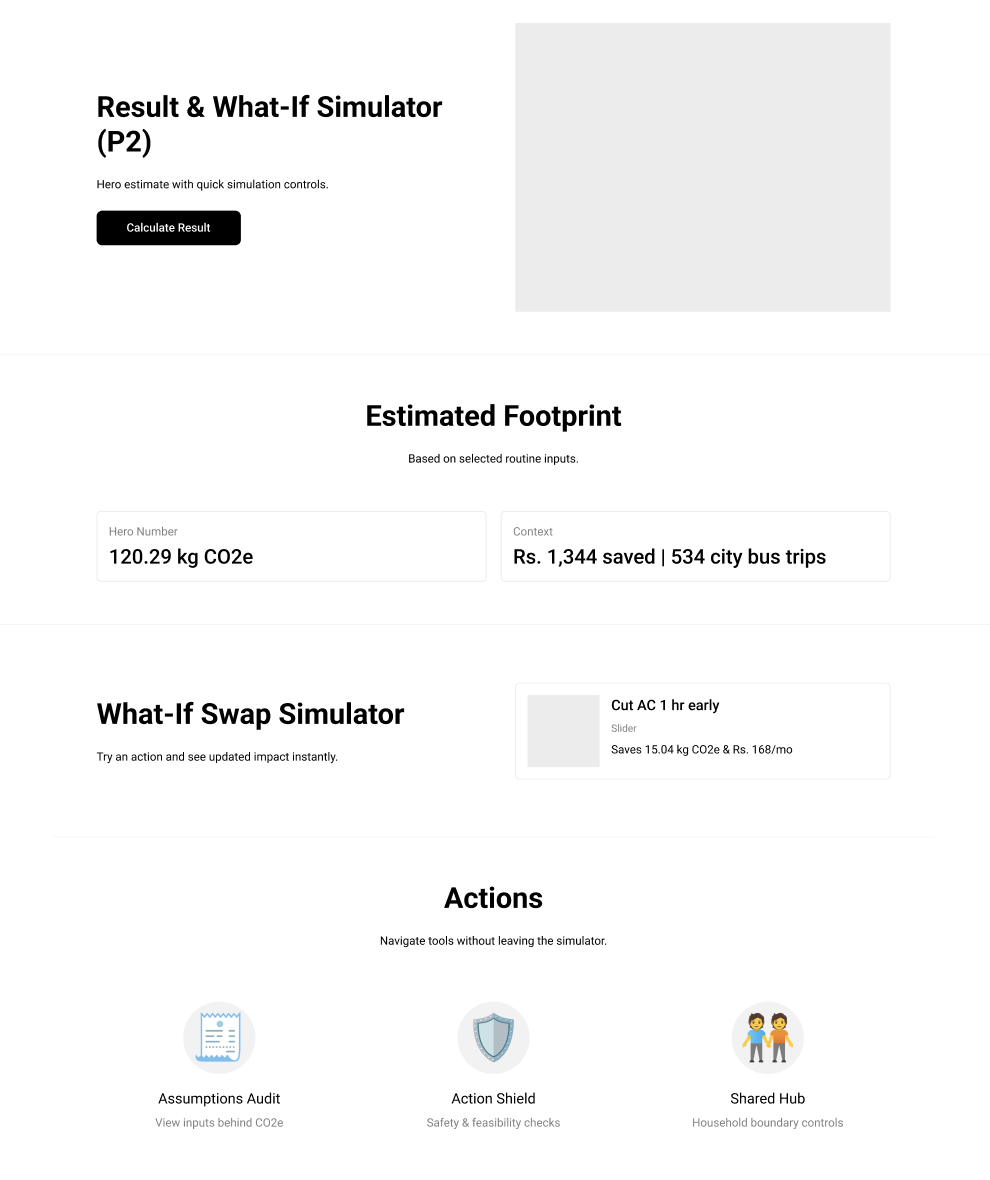
\includegraphics[width=0.5\linewidth]{pic4.png}
            \caption{Enter Caption}
\begin{figure}
                \centering
                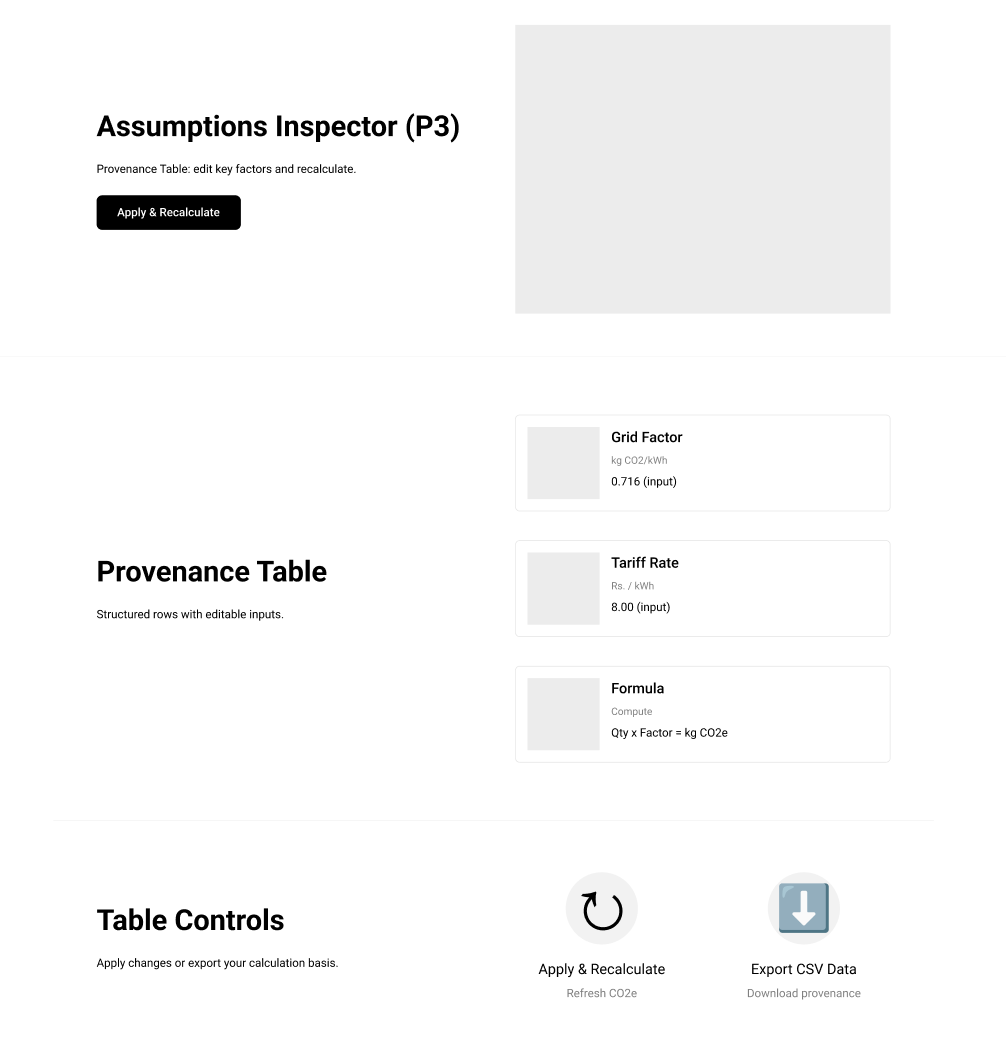
\includegraphics[width=0.5\linewidth]{pic5.png}
                \caption{Enter Caption}
\begin{figure}
                    \centering
                    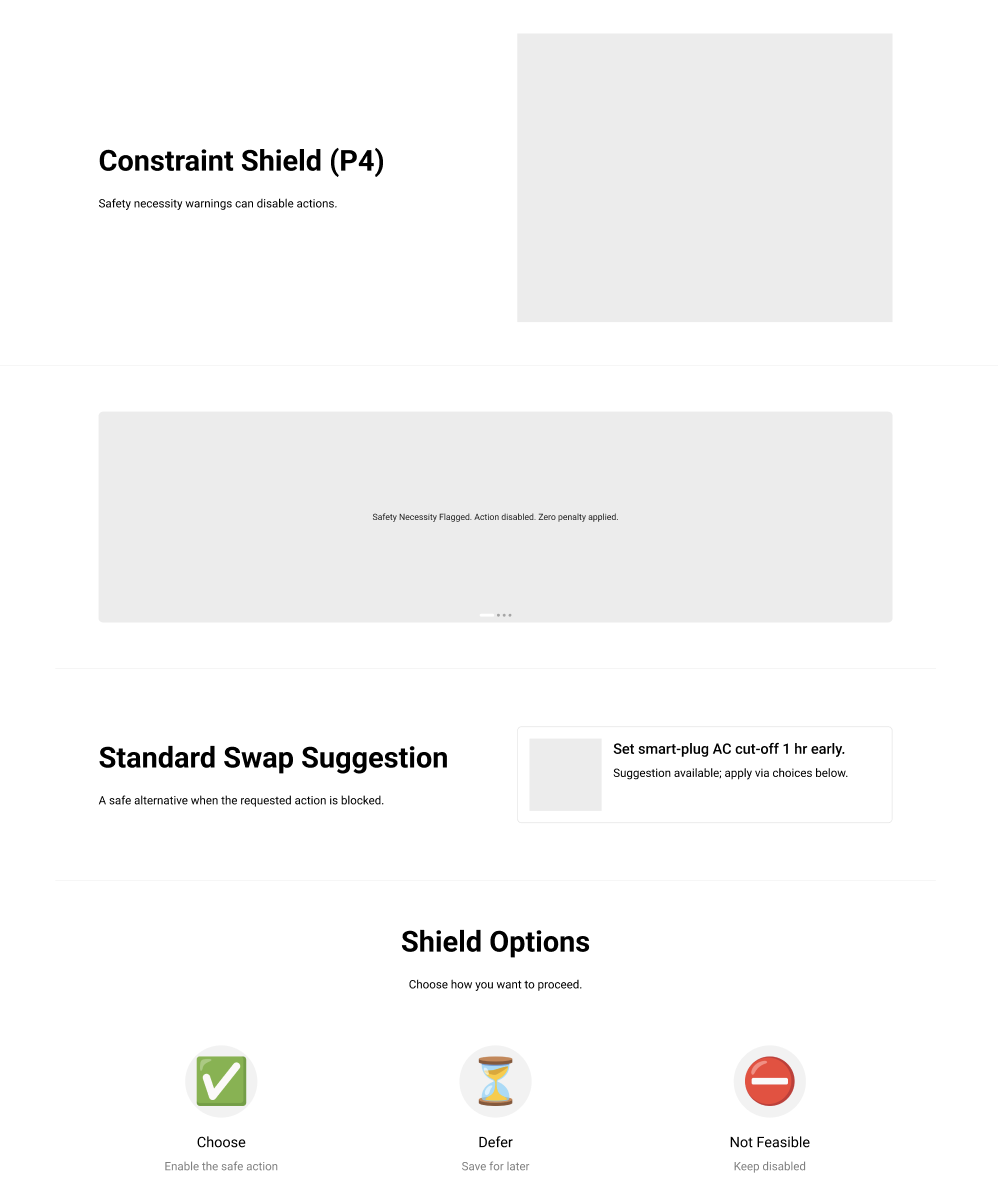
\includegraphics[width=0.5\linewidth]{pic6.png}
                    \caption{Enter Caption}
\begin{figure}
                        \centering
                        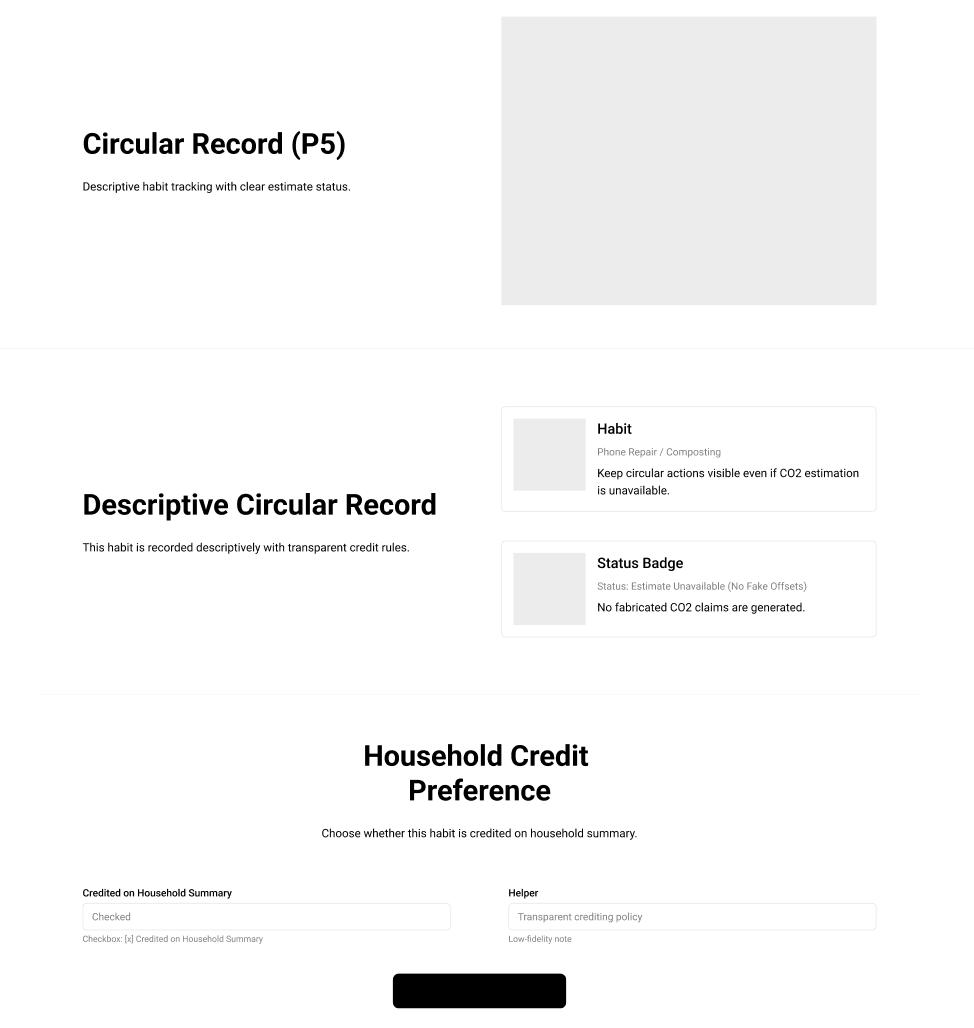
\includegraphics[width=0.5\linewidth]{pic7.png}
                        \caption{Enter Caption}
\begin{figure}
                            \centering
                            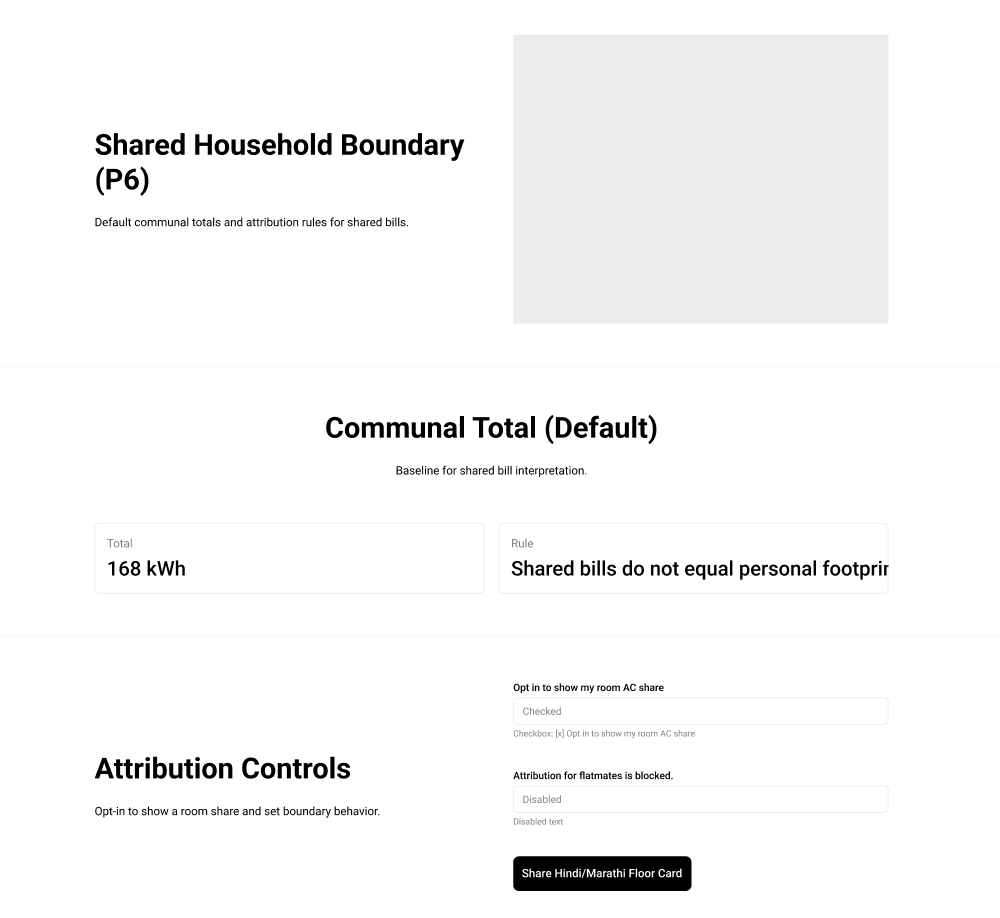
\includegraphics[width=0.5\linewidth]{pic8.png}
                            \caption{Enter Caption}
\begin{figure}
                                \centering
                                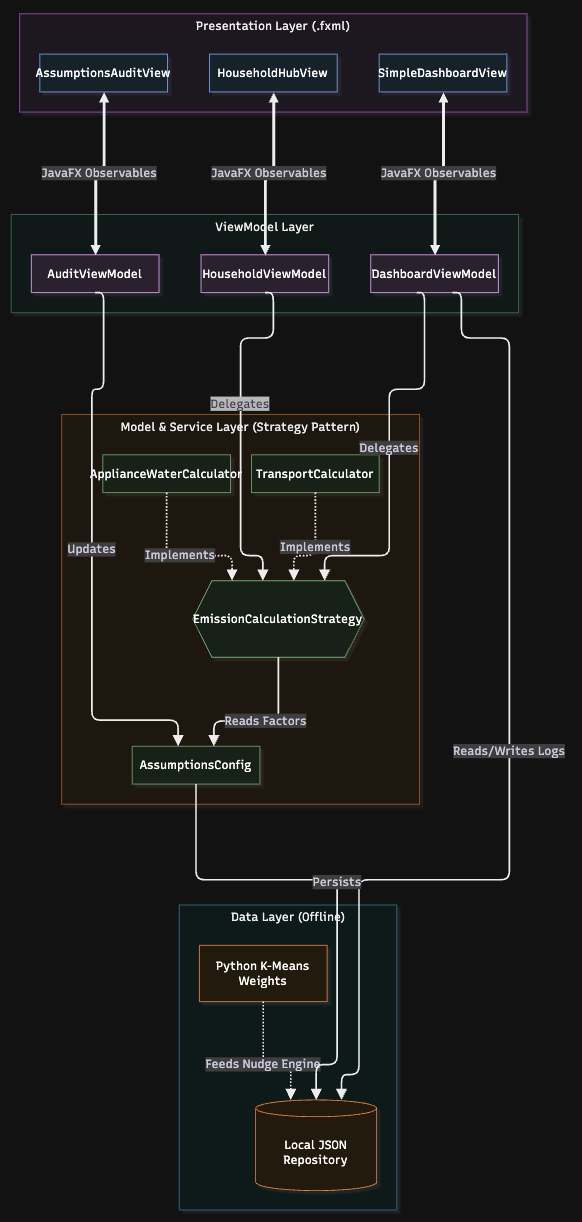
\includegraphics[width=0.5\linewidth]{pic9.png}
                                \caption{Enter Caption}
                                \label{fig:placeholder}
                            \end{figure}
                                                        \label{fig:placeholder}
                        \end{figure}
                                                \label{fig:placeholder}
                    \end{figure}
                                        \label{fig:placeholder}
                \end{figure}
                                \label{fig:placeholder}
            \end{figure}
                        \label{fig:placeholder}
        \end{figure}
                \label{fig:placeholder}
    \end{figure}
        \label{fig:placeholder}
\end{figure}
